\chapter[Effect of resonances on the detectability of EMRIs]{Effect of resonances on the detectability of extreme-mass-ratio inspirals}\label{ch:effect-resonances}

One of the targets of pre-eLISA research is to generate a bank of waveform templates, $h(t;\boldsymbol{\lambda})$ described by some set of parameters $\boldsymbol{\lambda}$. Once observational data, $s(t)$, has been collected, we can then search over the template bank to find the model that most closely matches the data. In order for the best-fit model to have any physical significance, we require that the waveform templates accurately reproduce what we expect to observe in nature. However, they cannot be too computationally expensive, as this would prohibit an effective search over the parameter space.

Ideally, we would like to use waveform templates from EMRI systems that are evolved under the action of the full gravitational self-force. Such a computational scheme is not yet available and so we are forced to use waveforms computed under the adiabatic approximation. We know that this explicitly eliminates any effects of transient resonances but it is unclear how that impacts the detectability of EMRIs using adiabatic templates. To assess this, we compare simulated data $s(t;\bar{\boldsymbol{\lambda}})$ generated using the instantaneous self-force model, with templates $h(t;\boldsymbol{\lambda})$ generated using the 2-torus-averaged adiabatic model, detailed in \secref{res-ad-averaging}.

\section{Gravitational wave generation}
To generate gravitational waveforms, we choose to employ the NK method of \citet{babak_kludge_2007}. As discussed in \secref{EMRI-GWs}, the principle behind the class of kludge methods is to first compute inspiral trajectories and then separately (and not necessarily consistently) calculate the GW emission sourced by a compact object moving along that trajectory. This can be much quicker and easier to calculate than waveforms using Teukolsky-based methods and yet gives similar results.

Following the NK method, we first compute the inspiral trajectory of the compact object using the method of osculating elements detailed in \secref{EMRI-evolution-scheme}. We then interpret the Boyer--Lindquist coordinates as spherical polar coordinates in Minkowski, facilitating the use of a flat-spacetime waveform generation technique. Specifically, we apply the standard quadrupole formula. We expect these waveforms to be sufficiently accurate for our purposes, given the inaccuracy of the self-force model being employed. It would, however, be straightforward to adopt a different waveform generation scheme, for example by including higher order multipole moments, should advances be made in determining the self-force.

Once we have established a waveform generation procedure, we can define a natural inner product between two waveforms, $s_\alpha(t)$ and $h_\alpha(t)$, where the subscript $\alpha$ refers to different detector outputs. Following \eqnref{noise-overlap}, we write
\begin{equation}
\label{eq:effres-innerprod}
\innerii{s}{h} = 2 \sum_\alpha \intd{0}{\infty}{\frac{\tilde{s}_\alpha(f)\tilde{h}_\alpha^*(f)+\tilde{s}_\alpha^*(f)\tilde{h}_\alpha(f)}{S_{n,\alpha}(f)}}{f},
\end{equation}
where $\tilde{s}_\alpha(f)$ represents the Fourier transform of $s_\alpha(t)$, similarly for $\tilde{h}_\alpha(f)$, and $S_{n,\alpha}(f)$ is the one-sided noise PSD for detector $\alpha$. Given a specific data realisation, we can evaluate the signal-to-noise ratio (SNR) for each waveform template, defined by
\begin{equation}
\rho\left[h\right] = \frac{\innerii{s}{h}}{\sqrt{\innerii{h}{h}}}.
\end{equation}
If a template were to exactly match the data, it would produce an SNR of $\sqrt{\innerii{s}{s}}$ and so the overlap
\begin{equation}
\label{eq:effres-overlap}
\mathcal{O}\left[h\right] = \frac{\innerii{s}{h}}{\sqrt{\innerii{s}{s}}\sqrt{\innerii{h}{h}}}
\end{equation}
provides an indication of how well-matched the template is to the data. 

We are interested in the detectability of EMRIs using future space-based GW detectors and so we use a PSD appropriate for describing the eLISA mission concept, specifically choosing the analytic approximation of \citet{amaro-seoane_low-frequency_2012}. We compute two orthogonal detector responses corresponding to the two GW-sensitive datastreams of a 6 laser link eLISA mission, and carry out the appropriate sum over these outputs according to \eqnref{effres-innerprod}. For brevity, we shall henceforth drop the subscript $\alpha$.

In practice, the continuous functions $s(t)$ and $h(t)$ are not available, instead replaced by the time series $s(t_i)$ and $h(t_j)$ where $\{t_i\}$ and $\{t_j\}$ are equally-spaced sets of time values, but which do not necessarily have the same length or spacing. To account for this, when evaluating overlaps, we first project the $h(t_j)$ onto $\{t_i\}$ using a cubic interpolation scheme, setting any values outside the domain of $\{t_j\}$ to zero. A Planck-taper window function \citep{mckechan_tapering_2010} is applied to the resulting time series. This can be defined in a continuous form by
\begin{equation}
w(t) = \left\{
\begin{array}{ll}
	0 & t\leq t_1 \\
	\left(1+\exp\left(\frac{t_2-t_1}{t-t_1}+\frac{t_2-t_1}{t-t_2}\right)\right)^{-1} & t_1 < t < t_2 \\
	1 & t_2\leq t\leq t_3 \\
	\left(1+\exp\left(\frac{t_3-t_4}{t-t_3}+\frac{t_3-t_4}{t-t_4}\right)\right)^{-1} & t_3 < t < t_4 \\
	0 & t_4\leq t,
\end{array}\right.
\end{equation}
where $t_1$ and $t_4$ are chosen to encompass the whole waveform and $t_2$ and $t_3$ are the times of the second closest stationary points to each end, ensuring that the transition is not too sharp; the smoothness of the waveform at each end reduces unwanted spectral leakage in the Fourier transforms.

After tapering the projected waveforms, we then calculate inner products according to \eqnref{effres-innerprod}, using discrete Fourier transforms and replacing the integral over frequency with an appropriate sum over Fourier modes. In addition, we maximise every overlap calculation with respect to some time-offset between the models by finding the maximum value of the cross-correlation between the waveforms. This process can be performed cheaply using Fourier transforms and can provide a significant increase to the overlap, even though typical offset times are shorter than the orbital timescale.

We demonstrate our waveform generation using the illustrative system introduced at the end of \secref{res-ad-averaging}. Once the trajectories have been computed using both the instantaneous and adiabatic evolutions, we can calculate the corresponding waveforms. The plus-polarised GW at the start and end of the evolution is shown in \figref{good-waveform}. The waveforms show good agreement in both amplitude and phase; we find an overlap of $0.993$, illustrating that adiabatic models can be used in place of the instantaneous evolution in cases where resonances are not encountered.

\begin{figure}[htbp]
\centering
\includegraphics[width=\textwidth]{good_waveform}
\caption{\label{fig:good-waveform}The plus-polarised waveform for an illustrative EMRI system with $p=7.5$, shown for two short segments at the start (left plot) and end (right) of a $2$ year evolution. The instantaneous (thick blue line) and adiabatic (thin golden line) models are both shown, but are indistinguishable by eye.}
\end{figure}

\section{The effect of transient resonances on a single system}
\label{sec:effres-single-system}
The illustrative EMRI system of the previous section does not encounter a significant resonance and the adiabatic evolution provides a good match to the instantaneous evolution. We now study a system that does pass through a resonance during its $2$ year evolution.

\subsection{Dephasing}
\label{sec:effres-dephasing}
We choose the initial conditions to be the same as before but with an initial semi-latus rectum $p=7.85$. This system passes through the 2:3 resonance, the effect of which is to cause a shift in the orbital parameters (and hence in the fundamental frequencies) that is not replicated by the adiabatic evolution, thus resulting in a rapid dephasing of the waveforms. Plotting the plus-polarised GWs at the start and end of the evolution, as before, demonstrates this dephasing; the waveforms are shown in \figref{dephased-waveform}.

\begin{figure}[htbp]
\centering
\includegraphics[width=\textwidth]{dephased_waveform}
\caption{\label{fig:dephased-waveform}The plus-polarised waveform for an illustrative EMRI system with $p=7.85$, shown for two short segments at the start (left plot) and end (right) of a $2$ year evolution. The instantaneous (thick blue line) and adiabatic (thin golden line) models are both shown; there is a significant dephasing between them by the end of the evolution.}
\end{figure}

To highlight the dephasing more quantitatively, we calculate the shortened overlap between the two models as a function of time, $t$. We define this as the overlap obtained by including only the part of the waveform within some $\Delta t$ of $t$. For our illustrative system, we choose $\Delta t$ such that we can calculate 25 non-overlapping values of this shortened overlap. Before the resonance occurs, the adiabatic model provides a good match to the instantaneous evolution but the overlap is reduced near to the resonance and never fully recovers afterwards. This is shown in \figref{overlap-dephasing}, which is centred on the time at which the instantaneous evolution crosses the 2:3 resonance.

\begin{figure}[htbp]
\centering
\includegraphics[width=0.92\textwidth]{overlap_vs_time}
\caption{\label{fig:overlap-dephasing}The overlap computed between the instantaneous evolution and an adiabatic evolution for an illustrative EMRI system with $p=7.85$, as a function of time, including only the parts of the waveforms within some $\Delta t$ of $t$, arbitrarily chosen to give 25 independent (non-overlapping) calculations. The time axis is centred on the value at which the instantaneous evolution crosses the 2:3 resonance.}
\end{figure}

Also shown is the shortened overlap computed using a different adiabatic evolution that is chosen to match the instantaneous evolution at the end of the observation. In this case, we see similar behaviour as before: the adiabatic waveform has a high overlap in the region where it is constructed to match the instantaneous evolution; and the boundary of that region is set by the location of the 2:3 resonance.

\subsection{A one-parameter family of adiabatic evolutions}
\label{sec:effres-1p-family}
To be able to quantify the effect that resonances have on EMRIs, we wish to use the full overlap between the instantaneous and adiabatic models computed for the entire length of the observed inspiral. The dephasing means that an adiabatic evolution with the same initial conditions is likely to have a low overlap if a significant resonance is encountered. However, this does not necessarily mean that all adiabatic evolutions have low overlaps; we need to search for optimal adiabatic parameters that maximise the overlap.

The large parameter space of waveforms, coupled with the expensive nature of our 2-torus averaging routine, renders a brute force approach computationally unfeasible. It is therefore necessary to restrict the search in some way. As a preliminary investigation into the importance of resonances, we do this by focussing on a small subset of parameters that we suspect will produce a large overlap. We make the assumption that a good adiabatic model will \emph{exactly} match the instantaneous model at some time $t_{\mathrm{match}}$. This reduces the search to a one-parameter family of waveforms that can easily be computed concurrently with the instantaneous evolution.

The problem of searching over adiabatic templates now reduces to the task of choosing appropriate values of $t_{\mathrm{match}}$. Anticipating that resonances shall play a key role in determining the extent of waveform overlap, we choose matching times situated $5\tau_\mathrm{res}$ after each resonance of interest; we focus on the low-order 2:3 and 1:2 resonances as we expect these to be the most significant. These matching times lie in a portion of the evolution that is not affected by a resonance and so should result in a large overlap for that region of the inspiral. We also include templates that match at the start of the evolution, so that we have a model that should match the portion of the evolution before the first resonance, and at the end of the evolution, as this is often where most SNR is accumulated. In addition, we include models that match exactly on each of the resonances as these may achieve partial matching both before and after the resonance and hence perform well.

In our experience, we found that these choices were not sufficient to produce a good family of adiabatic waveforms. In particular, if an adiabatic model happened to match the instantaneous model close to the edge of the envelope generated by the fast orbital evolution, then the two trajectories eventually diverged and the resulting waveform provided a poor match. We therefore adjust the values of $t_{\mathrm{match}}$ so that they correspond to times of apoapsis. This ensures that the adiabatic model intersects with the instantaneous model close to the centre of the envelope, as demonstrated by the inset plots in \figref{good-traj}. As a result, we obtain much higher overlaps in general.

We have tried a more rigid system of choosing the values of $t_{\mathrm{match}}$, producing an adiabatic evolution regularly at fixed intervals, but these generally perform no better than our adaptive match points and require many more adiabatic evolutions to be calculated.

This one-parameter family of adiabatic models does not explore the extrinsic parameter space nor does it consider different values of the constant intrinsic parameters (the masses of the BHs and the central BH spin). It is possible that small deviations from these true parameters give rise to better matching adiabatic models, to partially correct for the (lack of) resonance effects. Indeed, systematic biases in parameter estimation are expected when the model waveforms do not accurately reflect the data \citep{cutler_lisa_2007}. The result of these restrictions is that the maximum overlap calculated using our family is a strict lower bound on the true maximum overlap.

\subsection{Loss of signal-to-noise ratio}
For the illustrative EMRI system detailed in \secref{effres-dephasing}, we have computed the family of adiabatic models set by $t_{\mathrm{match}}$ and the resulting trajectories are consistent for the length of the evolution. As they cannot be easily distinguished by eye, we plot the difference (in $E$, $L_z$ and $Q$) between each model and the adiabatic evolution that matches at the start, shown in \figref{res-diff-traj}. The jumps in the orbital parameters due to the 2:3 resonance can be clearly seen, as can the fast orbital oscillations present in the instantaneous evolution but absent in the adiabatics.

\begin{figure}[htbp]
\centering
\includegraphics[width=\textwidth]{res_diff_traj}
\caption{\label{fig:res-diff-traj}The differences in orbital parameters $E$ (upper plot), $L_z$ (middle) and $Q$ (lower) between each evolution scheme and the adiabatic model that matches at the start. The solid line shows the instantaneous evolution and the dashed lines show the different adiabatic evolutions, which match the instantaneous evolution at different times throughout the inspiral (numbers in parentheses give the overlap with the full evolution): at the start (0.207), at the 2:3 resonance (0.432), after the 2:3 resonance (0.258) and at the end (0.677).}
\end{figure}

None of the adiabatic models presented here give a particularly high overlap with the instantaneous evolution due to the effects of the resonance. The best-performing adiabatic model was that which matched at the end, giving $\mathcal{O} = 0.677$, while the model that matches at the start gives only $\mathcal{O} = 0.207$.

\subsection{Effect of orbital parameter jumps}
\label{sec:effres-jumps}
The magnitude of the resonance jump depends sensitively on the relative phase of the $r$ and $\theta$ motions. In order to fully understand the effect of resonances on the recovered overlap, it is instructive to study the resonance problem using an ensemble of systems differing only in the initial value of the radial phase $\psi_0$, as carried out previously in \secref{res-orb-jumps}. Here we use our illustrative system instead, computing the trajectories and waveforms for $100$ values of $\psi_0$, uniformly sampled from $[0,2\pi)$.

For each system, we calculate the size of the resonance jump for $E$, $L_z$ and $Q$. According to \eqnref{res-jump}, these values should be oscillatory with respect to a \emph{single} phase parameter $q_0$. Therefore, plotting the jumps of one parameter against another should produce an ellipse.\footnote{We expect an ellipse rather than a simple linear dependence since the jumps in different parameters may have a phase offset with respect to each other.} Choosing an arbitrary zero-point around the ellipse, we may extract a phase parameter $q$ for each system; this is linearly offset from $q_0$ due to the choice of zero-point. We obtain the same value of $q$ irrespective of which two resonance jumps are used, lending support to the form of \eqnref{res-jump} and giving us confidence in our numerical jump calculations. The relative orbital parameter jumps are shown for each system in \figref{res-jump-vs-q}, as a function of $q$, along with sinusoidal fits to the data. The jumps in $E$ and $L_z$ are approximately in phase, but those in $Q$ are found to be offset; this means that for every value of $q$, there is always a resonance jump in at least one parameter.

\begin{figure}[htbp]
\centering
\includegraphics[width=0.92\textwidth]{res_jump_vs_q}
\caption{\label{fig:res-jump-vs-q}The magnitude of the relative orbital parameter jump for our illustrative system as a function of the extracted phase parameter $q$. The individual jumps as well as a sinusoidal fit are plotted for $E$ (blue circles), $L_z$ (gold squares) and $Q$ (green triangles).}
\end{figure}

After extracting the value of $q$, we compute the overlap between the instantaneous waveform and the family of adiabatics given by our set of match times $t_\mathrm{match}$ described in \secref{effres-1p-family}. The largest overlap in each case, plotted in \figref{overlap-vs-q}, appears to be roughly independent of the value of $q$ and hence with the relative sizes of the orbital parameter jumps.

The best performing adiabatic for the majority of our systems matched at the end of the inspiral. We can therefore estimate the value of the overlap by assuming that the adiabatic waveforms recover the entire SNR in the region post-resonance, but none at all in the region pre-resonance. We expect the overlap to scale with the fraction of time spent post-resonance,\footnote{The overlap is linear in the inner product $\innerii{s}{h}$ and so scales linearly with time. This is in contrast to the norm of a waveform $\innerii{s}{s}^{1/2}$, which scales with the square-root of time, as shown by \eqnref{EMRI-SNR-estimate}.} the value of which is demonstrated by the red line in \figref{overlap-vs-q}. There is not an exact equivalence because of the frequency-dependent noise of eLISA; cycles near the end of the inspiral accumulate proportionally more SNR at a frequency closer to the minimum of the eLISA noise curve.

\begin{figure}[htbp]
\centering
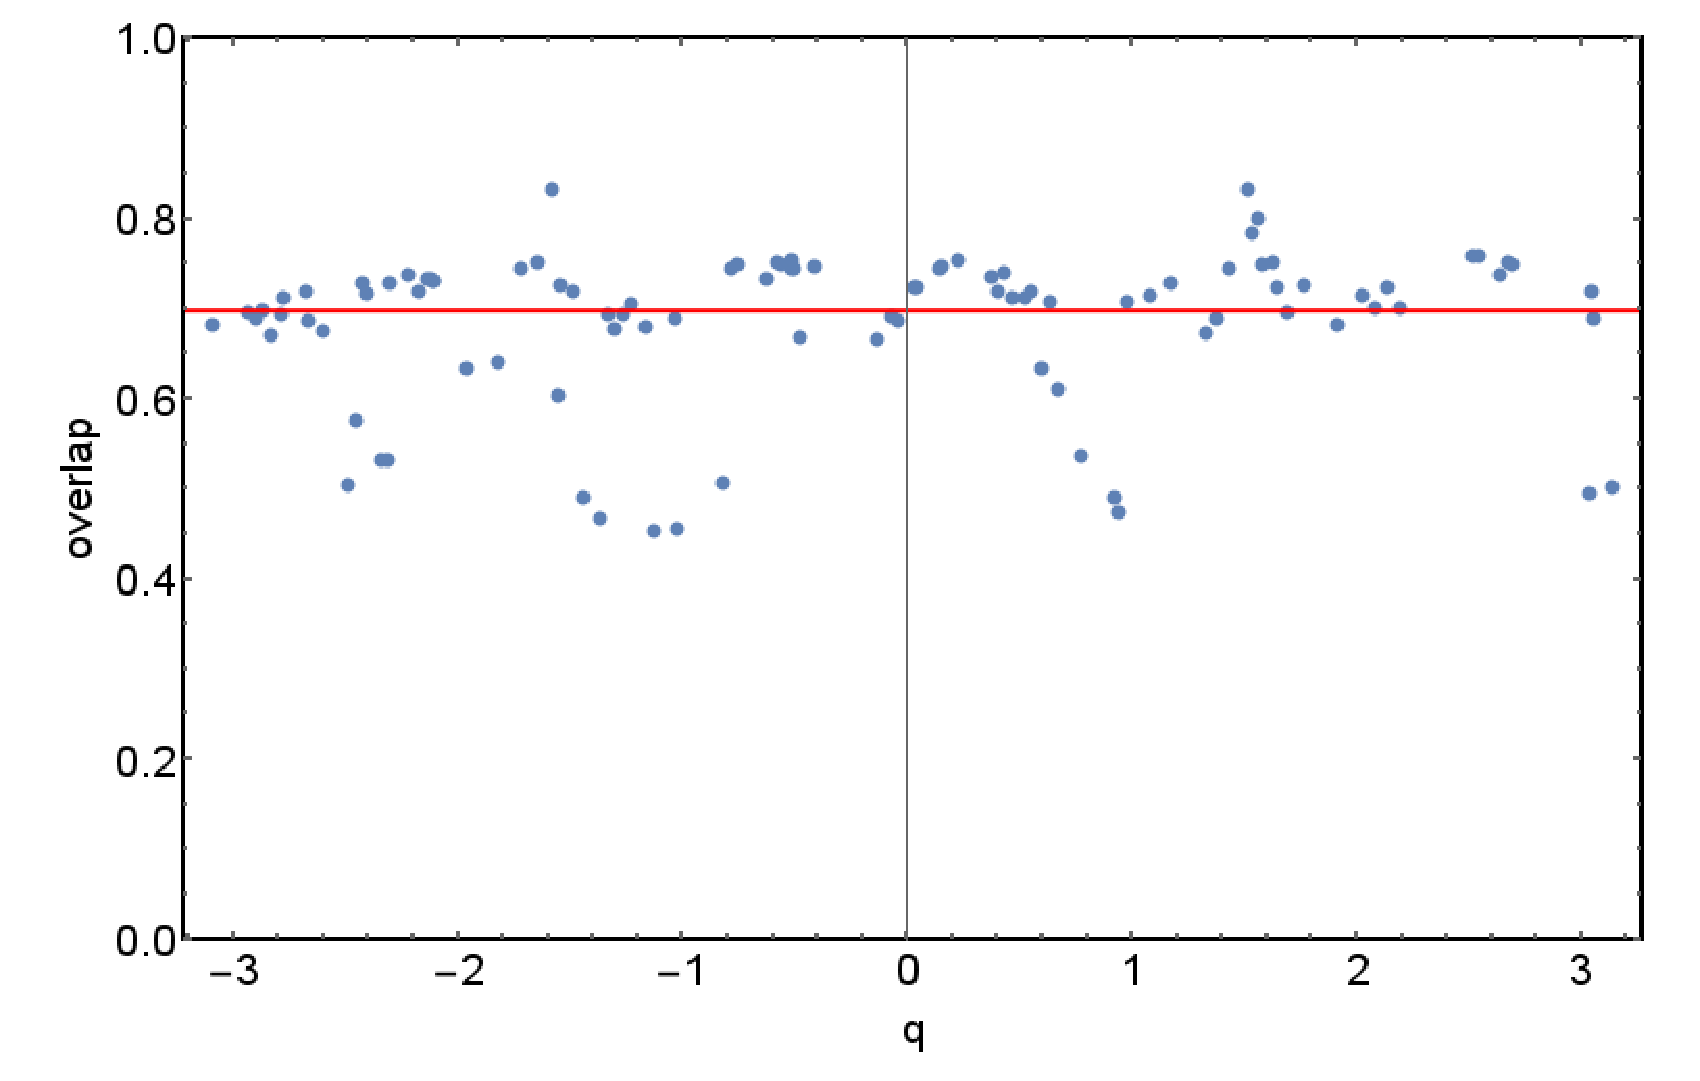
\includegraphics[width=0.92\textwidth]{overlap_vs_q}
\caption{\label{fig:overlap-vs-q}The overlap between the instantaneous and adiabatic evolutions, maximised over the family of generated adiabatics, as a function of the extracted phase parameter $q$. Each dot represents a system with our illustrative parameters and a random choice of the initial radial phase. The red line indicates the expected overlap assuming that the waveforms match exactly post-resonance, but have zero overlap pre-resonance.}
\end{figure}

Systems with $|q| \approx \pi$ (corresponding to small jumps in $E$ and $L_z$) have higher than average overlaps due to additional accumulation in the pre-resonance region. The adiabatic models of these systems dephase more slowly, but still do not produce very high overlaps due to the jump in $Q$. A small fraction of systems have a much lower overlap than expected, at around $0.5$. This is due to a sub-optimal choice of the matching times; making small adjustments to $t_\mathrm{match}$ can lead to higher overlaps, but the exact adjustments required are difficult to predict in advance.


\section{The effect of transient resonances on a population of systems}
\label{sec:effres-population}
Strong resonances can limit our ability to recover SNR from waveforms using adiabatic templates; they partition the inspiral, splitting up the total SNR into different adiabatic regions, which may be individually undetectable. In order to assess the impact of this on future GW missions, we need to analyse the waveforms from a population of detectable EMRIs.

In \secref{EMRI-detectability}, we produced an astrophysical EMRI population, and generated an approximate waveform for each system using the analytic kludge (AK) model of \citet{barack_lisa_2004}. Calculating SNRs assuming 6 laser links and using the eLISA noise PSD, we found $513$ detectable events from a total of $6333$, assuming an SNR threshold of $15$. We now analyse these $513$ systems using our instantaneous and adiabatic self-force models. The parameter distributions for the mass and spin of the SMBH, the orbital shape parameters, the redshift of the source, and the length of the observation $t_\mathrm{insp}$ are shown in \figref{EMRIpar-dists}, to be contrasted with the distributions of the $5820$ systems with an SNR less than 15, which are also shown.

We note that eccentric prograde orbits around SMBHs with larger spins tend to produce larger SNRs, due to the fact that the periapse in such systems can get much closer to the SMBH, and so the compact object experiences the strongest gravitational fields. This effect also causes the detectable EMRIs to have smaller values of $p$ at plunge, as observed in the distributions. Systems at higher redshifts start to become undetectable because the amplitude of the signal scales inversely proportional to the luminosity distance to the source, and by $z=1.5$, the distribution of detectable EMRIs with eLISA has essentially vanished. The mass distribution for detectable EMRIs is peaked such that the typical GW frequency occurs at the base of the eLISA noise PSD.

\begin{figure}[htbp]
\centering
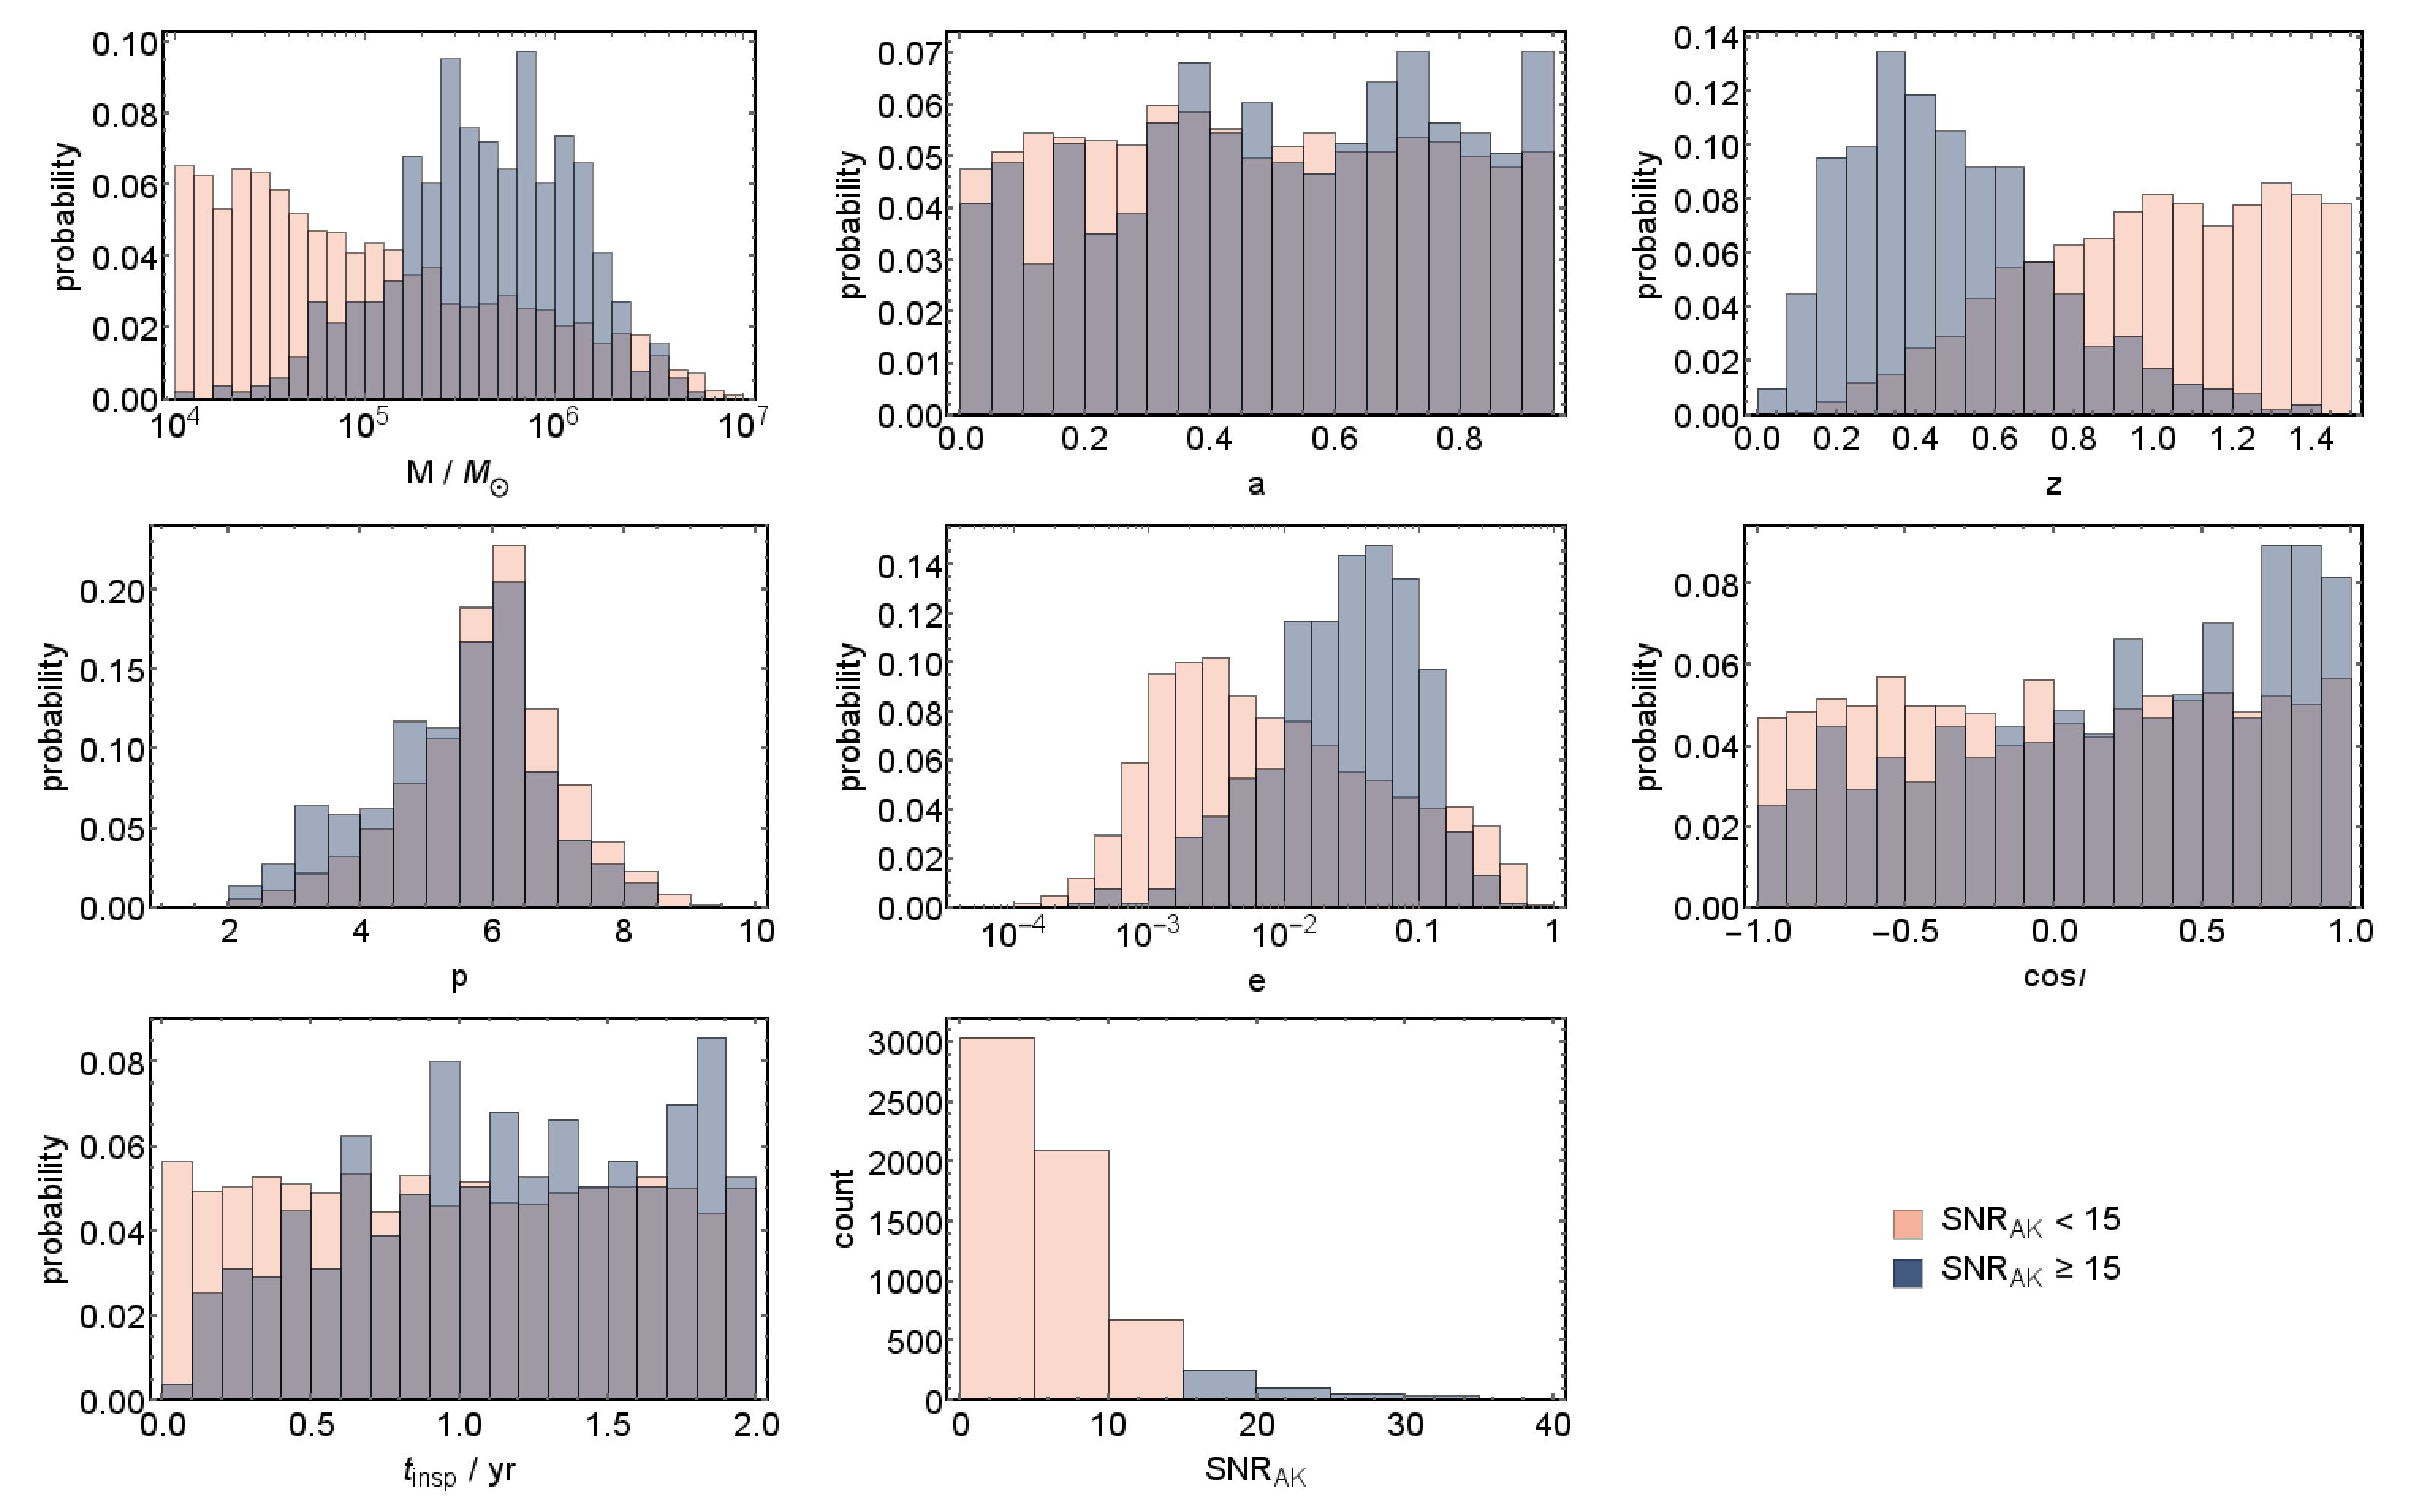
\includegraphics[width=\textwidth]{EMRIpar_dists}
\caption{\label{fig:EMRIpar-dists}The parameter distributions at plunge for our detectable EMRI systems (dark blue), alongside those of the undetectable systems (light pink). In each case, the y-axis values are the probability of a system being found in a particular bin, given that they are either detectable or undetectable. The exception to this is in the final plot for the SNR, where we show the number of systems in each bin. The SNRs quoted here are calculated using the AK model.}
\end{figure}

EMRI systems within our population tend to have small eccentricities at plunge due to the circularising effect of GWs: $85\%$ of detectable systems have $e < 0.1$, with a mean value of $0.05$ and a maximum of $0.4$. In \chapref{resonances}, we found a strong eccentricity dependence on the magnitude of the resonant flux enhancements. We therefore expect typical resonant jumps in these astrophysical systems to be much less than $1\%$, and so the resultant dephasing may be relatively weak.% We quantify this by calculating the loss of overlap in each system.

\subsection{Loss of signal-to-noise ratio}
After computing the SNRs of our NK waveforms for each of the $513$ systems, we can compare the values to those obtained in \secref{EMRI-detectability} using the AK formalism. The different approximation schemes are expected to produce different results, but they should be broadly similar. In \figref{pop-SNR-vs-eta}, we plot the ratio of the new SNR to the AK SNR, as a function of the mass ratio. We observe a clear trend, with systems closest to equal mass performing roughly as expected, but with the most extreme systems giving significantly lower SNRs.

This is a consequence of the PN self-force model we are using, which we have found overestimates the inspiral rate for EMRIs. Detectable systems with larger mass ratios (closer to equal mass) plunge at higher frequencies, and so during the 2 year observation window, they evolve within the bucket of the eLISA noise curve. Increasing the rate of evolution then does not significantly change the recovered SNR since we are still sensitive to all parts of the waveform. At smaller mass ratios, the systems evolve more slowly, from lower plunge frequencies. An increased evolution rate can shift the EMRI to outside the sensitive region of the detector, thus giving a much lower SNR.

\begin{figure}[htbp]
\centering
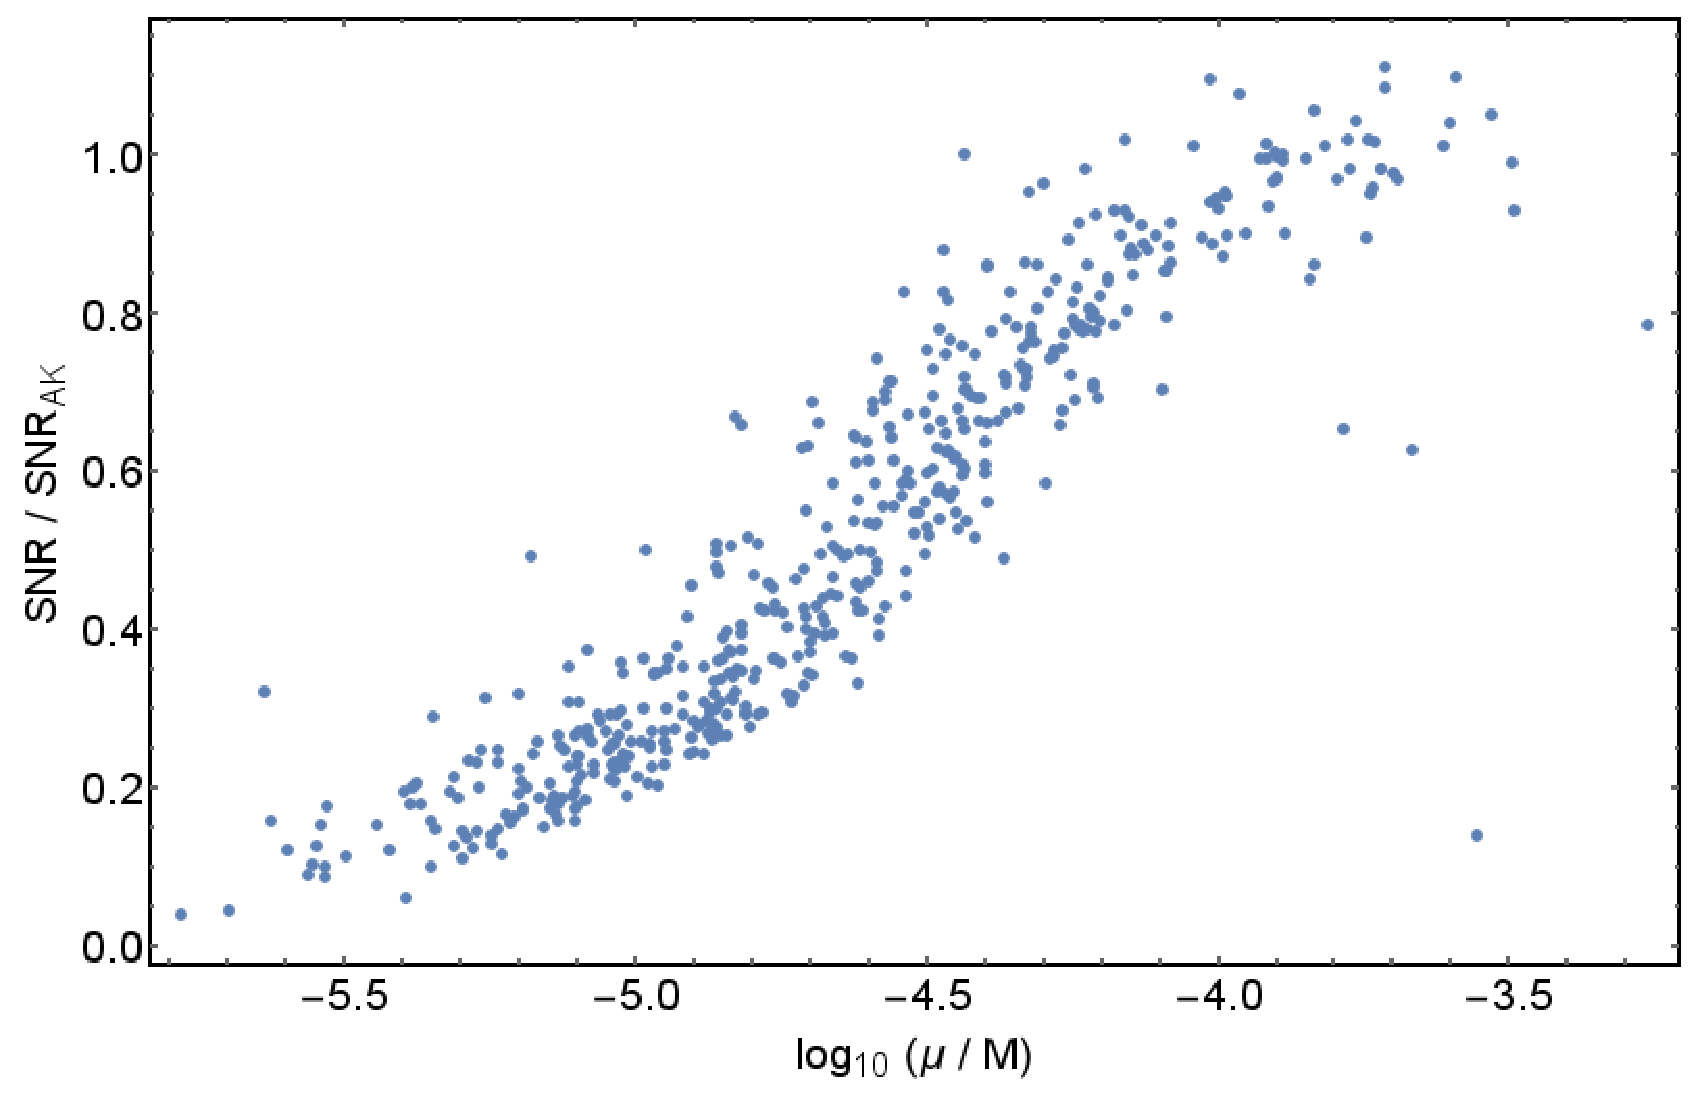
\includegraphics[width=0.92\textwidth]{pop_SNR_vs_eta}
\caption{\label{fig:pop-SNR-vs-eta}The ratio of SNRs as computed with waveforms generated using the NK (adopting our PN self-force model) and AK formalisms, as a function of (the base-10 logarithm of) the mass ratio. Each system has an AK SNR greater than 15, using the eLISA detector with 6 laser links.}
\end{figure}

Nevertheless, we may still study the effect of resonances, by comparing the maximum adiabatic SNR to the instantaneous SNR computed using the NK waveforms. The resulting overlap is still indicative of the effect of resonances on the population of systems.

\begin{figure}[htbp]
\centering
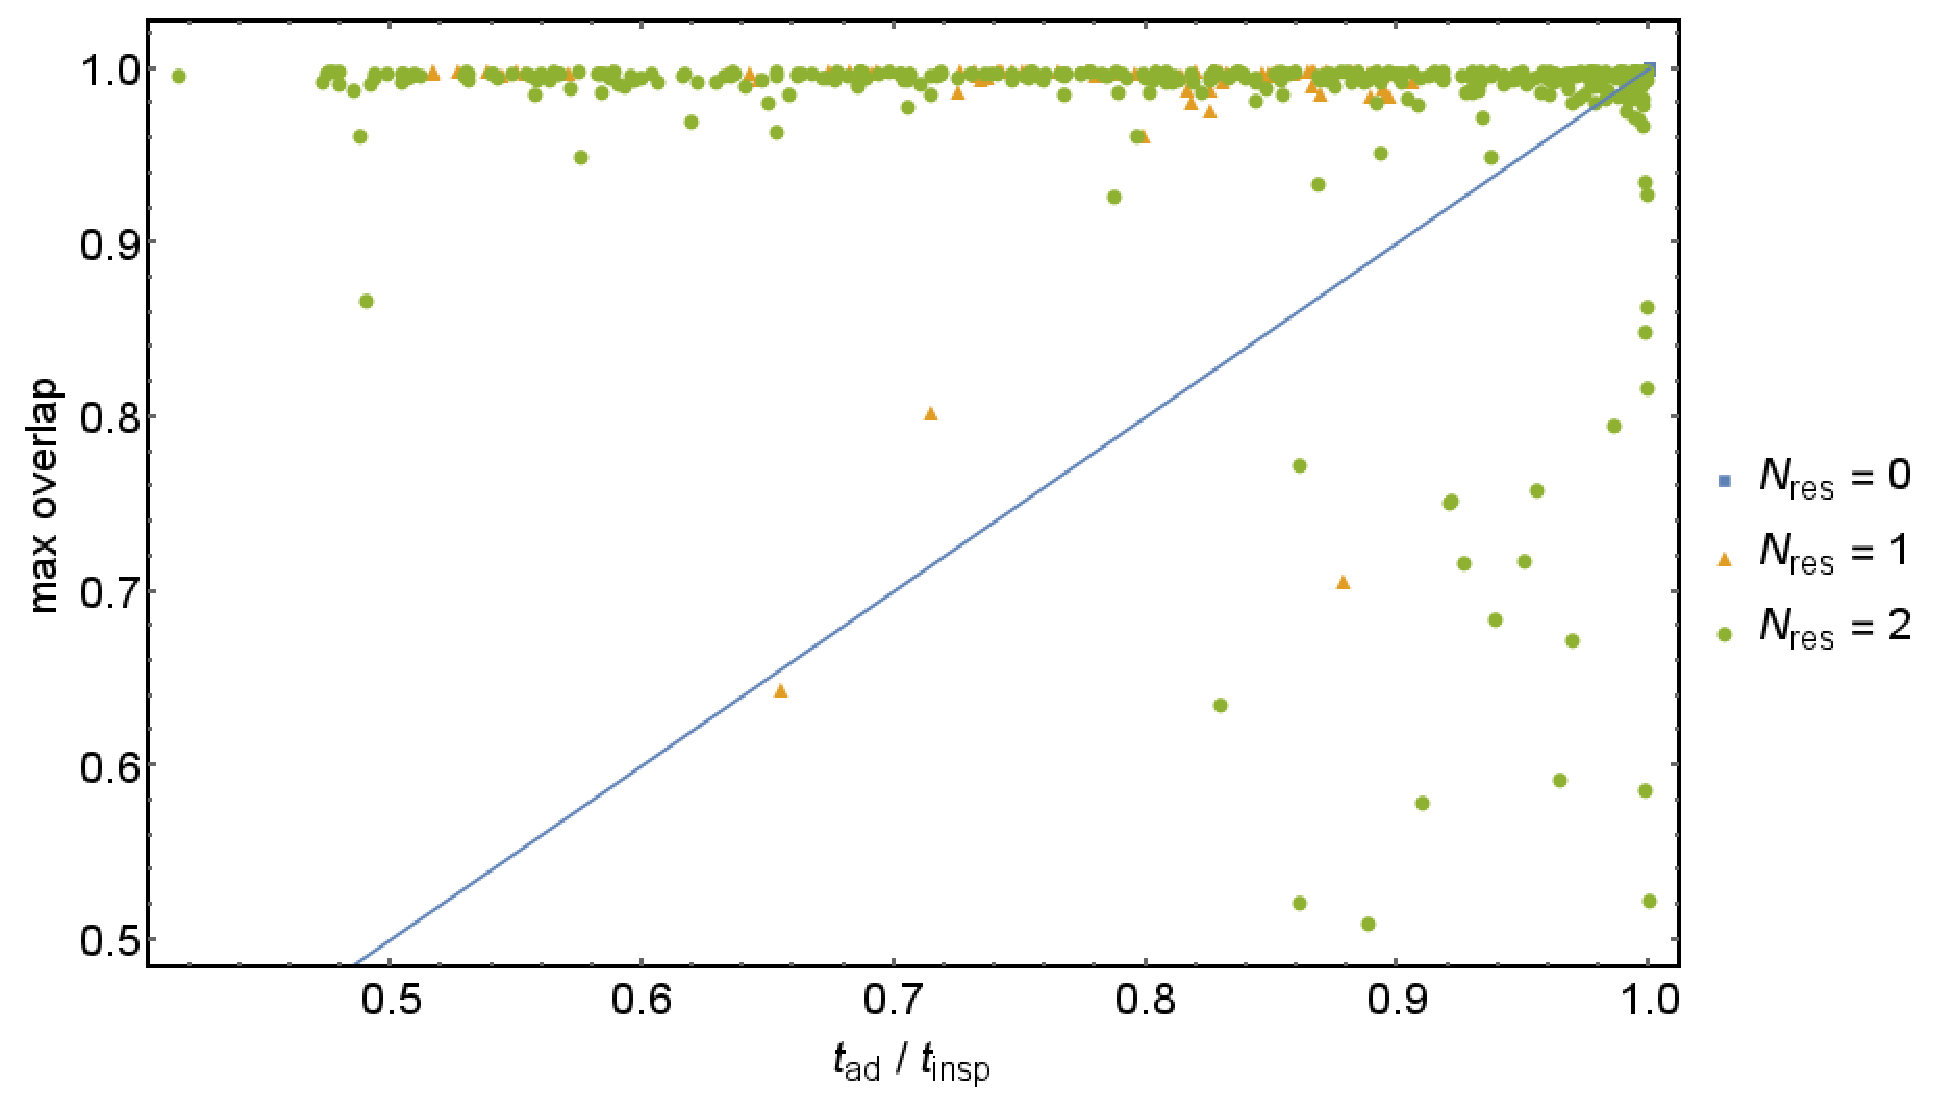
\includegraphics[width=0.92\textwidth]{pop_adSNR_vs_Tad}
\caption{\label{fig:pop-adSNR-vs-Tad}The maximum overlap for $513$ detectable EMRI systems obtained by comparing the instantaneous evolution with each of the adiabatic models in our one-parameter family. Each system encounters either $0$ (blue squares), $1$ (gold triangles) or $2$ (green circles) resonances during the observation window $t_\mathrm{insp}$. The overlap is plotted against the largest time spent by the inspiral without encountering any resonances $t_\mathrm{ad}$, normalised by $t_\mathrm{insp}$. The solid line corresponds to the expected value if the 1:2 and 2:3 resonances cause significant waveform dephasing.}
\end{figure}

We have calculated the longest period of time, $t_\mathrm{ad}$, during each inspiral, in which neither the 1:2 nor the 2:3 resonance occurs. From the results of \secref{effres-jumps}, we expect the recovered overlap to be approximately given by the proportion of time spent in a resonance-free region, that is $t_\mathrm{ad} / t_\mathrm{insp}$. In \figref{pop-adSNR-vs-Tad}, we plot the maximum overlap between the instantaneous and adiabatic models against this ratio, highlighting the number of resonances, $N_\mathrm{res}$, each system encounters. In the majority of cases, there is no significant impact on the recovered overlap using adiabatic models.

\begin{figure}[htbp]
\centering
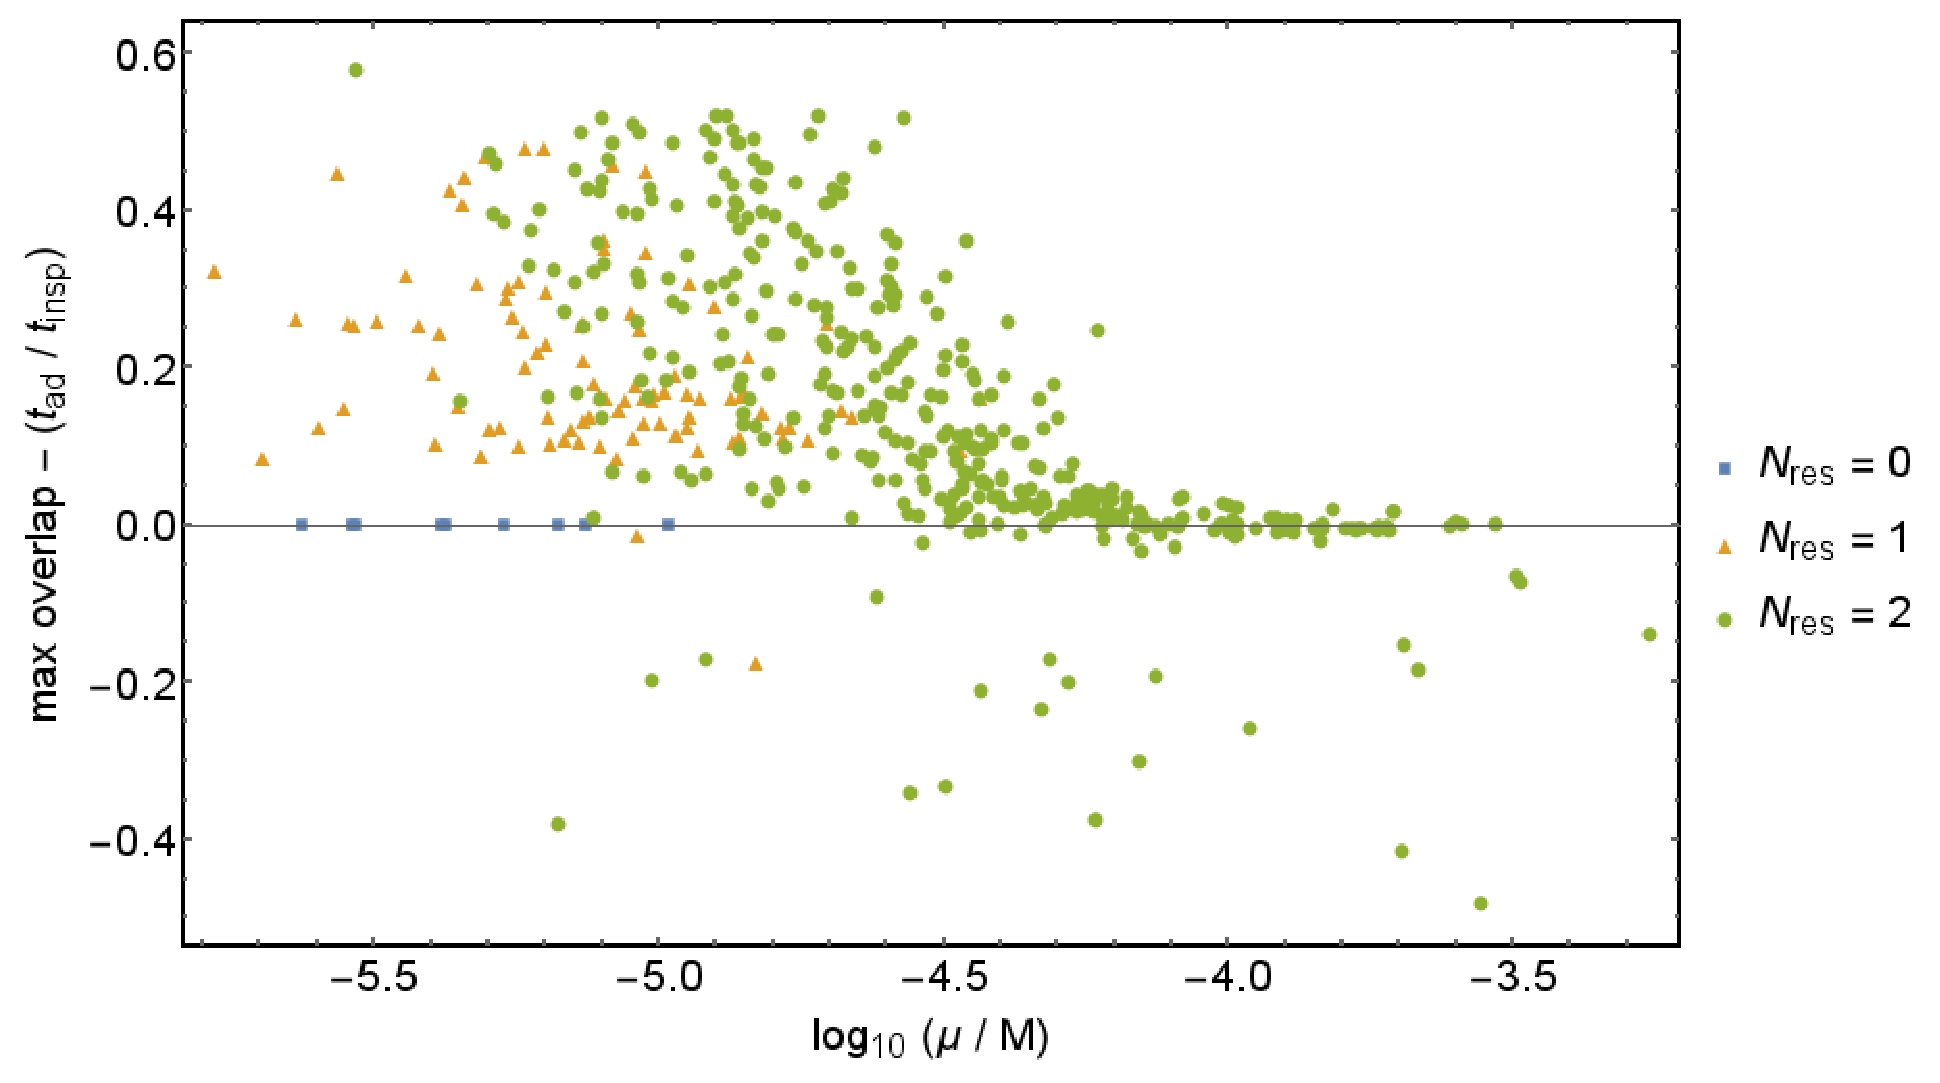
\includegraphics[width=0.92\textwidth]{pop_adSNR_vs_eta}
\caption{\label{fig:pop-adSNR-vs-eta}The difference between the maximum overlap and the expected value $t_\mathrm{ad} / t_\mathrm{insp}$, as a function of (the base-10 logarithm of) the mass ratio.}
\end{figure}

We can better understand the overlap distribution from \figref{pop-adSNR-vs-Tad} by considering the behaviour with the mass ratio. We do this in \figref{pop-adSNR-vs-eta}, plotting the difference between the computed maximum overlap and the value expected should resonances be important. A small proportion of systems have overlaps below the expected value (approximately $4\%$ have values less than $-0.05$). This might be caused by higher-order resonances disrupting the evolution, in which case $t_\mathrm{ad}$ should be smaller and the systems would lie on the expectation line. Alternatively, the low-order resonances might be long-lived, explaining why the recovered overlap is smaller than expected. However, a more likely explanation is that larger adiabatic overlaps are possible with models that we have not considered here (either with different values of $t_\mathrm{match}$ or outside our one-parameter family altogether).% We also suspect that the 2-torus averaging routine for some of these systems has not fully converged.

Roughly $30\%$ of the systems lie within $0.05$ of the expected value. However, the vast majority of these are not significantly disrupted by resonances, and produce overlaps approaching unity. For the smallest mass ratios, the inspiral rate is slow, and so the systems do not encounter either the 1:2 or 2:3 resonances during their lifetime. Meanwhile for the largest mass ratios, the EMRIs encounter both resonances very close to plunge. In each case, there is a long resonance-free region, allowing a high overlap to be recovered.

The remaining $66\%$ of systems have overlaps above the level expected if resonances were to play an important role. These occur at low and intermediate values of the mass ratio, where the inspiral rate is slow enough that the low-order resonances are encountered in the middle of the observation window, and the resulting value of $t_\mathrm{ad}$ is small. For these EMRIs, resonances are not as important as expected, which is likely due to the low eccentricities of our population leading to small (and in most cases, negligible) resonant flux enhancements.

Even if we assume that all overlap reductions are due to resonances (instead of due to our adiabatic family not being extensive enough) the overall effect on the population is not significant. To illustrate this, we plot the AK SNRs in \figref{pop-SNR-dist}, multiplied by the maximum recovered overlap to take into account the resonance behaviour. The total number of detectable systems using a threshold SNR of $15$ decreases from $513$ to $492$. If we increase the threshold, the fractional reduction in the number of detectable systems gets even smaller. We therefore conclude that resonances do not cause sufficient waveform dephasing across a population of EMRIs for the detection rate to be appreciably diminished.

%For the smallest mass ratios (below $\sim\mathcal{O}(10^{-5})$), the inspiral rate is slow, and so the systems are less likely to encounter the 1:2 or 2:3 resonances during their lifetime. Those that do not encounter either have a maximum overlap equal to unity, demonstrating that we can neglect the effect of higher-order resonances. Most of those that only encounter one resonance (specifically this is the 1:2 resonance, which occurs at smaller values of $p$ than the 2:3 resonance) also have overlaps close to $1$, suggesting that we may also neglect the 1:2 resonance for these systems.

%At intermediate values of the mass ratio (between $10^{-5}$ and $10^{-4.4}$), the EMRIs inspiral quickly enough to encounter both resonances within the observation time, but still give overlap values approaching $1$. There is more scatter in this case, but the overlaps remain significantly above the level expected if resonances were important. At the largest values of the mass ratio, the EMRIs encounter both resonances very close to plunge, resulting in a long resonance-free region. We can therefore always recover an overlap of approximately $1$.

%\footnote{The expected value $T_\mathrm{ad} / T_\mathrm{insp}$ used in \figref{pop-adSNR-vs-eta} is calculated assuming both the 1:2 and 2:3 resonances are significant. If we assume only the 2:3 resonance is significant, the predicted values will increase. However, we still compute overlaps that are higher than expected.}. We therefore conclude that neither the 1:2 nor the 2:3 resonance cause sufficient waveform dephasing to result in a significant loss of SNR.

%A small proportion of systems are not well-described by our family of adiabatic models: there are $23$ EMRIs with maximum overlaps less than $0.9$. Some of these are likely to have larger overlaps with adiabatics that we have not considered here (either with different values of $t_\mathrm{match}$ or outside our one-parameter family altogether). We also suspect that the 2-torus averaging routine for some of these systems has not fully converged. 

\begin{figure}[htbp]
\centering
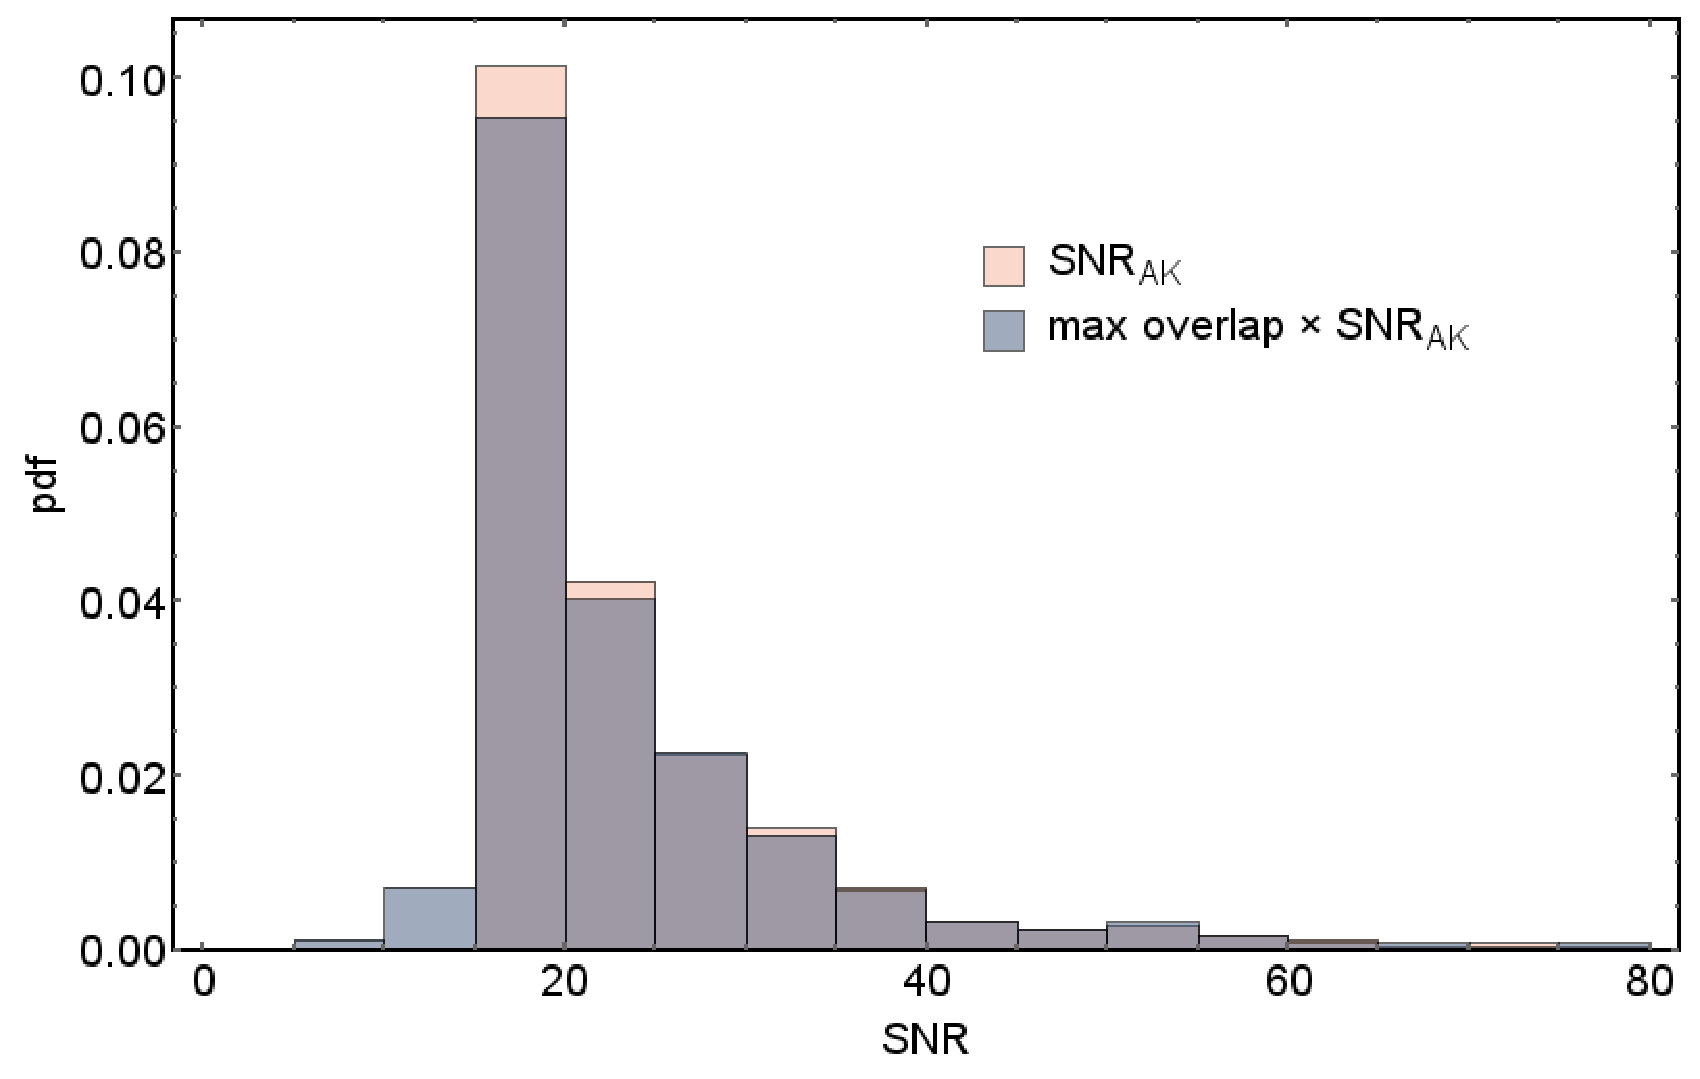
\includegraphics[width=0.92\textwidth]{pop_SNR_dist}
\caption{\label{fig:pop-SNR-dist}Histogram showing the probability distribution function for the detectable EMRI SNRs, as calculated using the AK formalism (light pink) and modified by the maximum adiabatic overlap (dark blue).}
\end{figure}

\section{Summary}
Tranisent resonances can cause severe dephasing in EMRI waveforms, with respect to adiabatic models that are indistinguishable away from the resonance. In \secref{effres-single-system}, we have shown that for one particular EMRI system with a high eccentricity, the resonant flux enhancements are large enough to shift the fundamental frequencies sufficiently that the waveforms promptly dephase. Using adiabatic models that exactly match the evolution at some time, the maximum recoverable overlap is given approximately by the fraction of time spent without encountering a resonance.

Despite this possibility of significant dephasing, we have found that the actual effect of resonances on a realistic population of EMRIs is minimal. For the most extreme mass ratios, the systems evolve too slowly to encounter resonances within the observation window. Detectable EMRIs that are the closest to equal mass evolve so quickly that the resonances occur very close to plunge. This means that the majority of the inspiral can be well-approximated by adiabatic models. Only systems with intermediate values of the mass ratio have the potential to be significantly disrupted by the presence of resonances, but we observe no such disruption. This can be attributed to the low eccentricities of our EMRI population, which give rise to small resonant flux enhancements.

Resonances may still play an important role in EMRI modelling. Our astrophysical population of EMRIs assumes one particular formation channel, which produces EMRIs that are close to circular at plunge. Different formation channels, such as the plunging orbits suggested by \citet{amaro-seoane_role_2013}, can produce populations with higher eccentricities, which may be impacted by resonance effects.


